Better forecasts can expand useful acceptance, but this alone does not specify how to spend the error budget. If a predictor's full-coverage risk is at most $r$, accepting all cases is a common optimum and mismatch disappears. Full-coverage risk above the cap is necessary for a strict objective reversal, but it is not sufficient: the same selective rule can still optimize both utilities (Appendix~\ref{app:necessity}). We test empirically whether reversal persists for the improved predictors here.

We use the three archived predictors and shared dates defined above in Appendix~\ref{app:accuracy}. Chronos-2 weights remain frozen \citep{ansari2025chronos2}; its selector is task-trained. This tests acceptance within each pipeline, not training-matched backbone superiority.

\begin{table}[H]
\centering\small
\caption{New retrospective comparison on the same 2,085,060 M5 development evaluation rows. Each predictor has a newly fitted error head; all share a newly fitted demand head, head-training rows, cap, and calibration dates. Higher coverage is better; lower WAPE is better. Full WAPE uses every row. These are fitted-policy outcomes, not population optima or a new external test.}
\label{tab:accuracy-selection}
\begin{tabular}{lrrrrr}\toprule
Predictor & Full WAPE & $\lambda$ & Rows (\%) & Demand (\%) & Accepted WAPE\\\midrule
Group-scaled L1 & 0.67139 & 1 & 85.90 & 80.59 & 0.63272 \\
Group-scaled L1 & 0.67139 & 0.25 & 80.13 & 86.06 & 0.63039 \\
Residual L1 & 0.65956 & 1 & 89.50 & 83.85 & 0.63298 \\
Residual L1 & 0.65956 & 0.25 & 86.48 & 89.72 & 0.63116 \\
Chronos-2 (raw) & 0.68310 & 1 & 80.74 & 75.42 & 0.63568 \\
Chronos-2 (raw) & 0.68310 & 0.25 & 75.39 & 81.82 & 0.63007 \\
\bottomrule\end{tabular}
\end{table}

The residual learner lowers full-coverage WAPE by 1.76\% relative to category-scaled L1. Both its row-weighted and mixed policies increase \emph{both} coverages over the corresponding base policies. Yet switching utility within that improved predictor still gains 5.87 demand-coverage points while losing 3.02 row points. The paired item-bootstrap intervals are $[4.84,6.88]$ and $[-3.57,-2.43]$ points, respectively. The same signs occur for the base and Chronos predictors, and for all three pure-demand endpoints (Appendix Table~\ref{tab:accuracy-ci}). These are retrospective, fit-conditional comparisons.

\begin{figure}[t]
\centering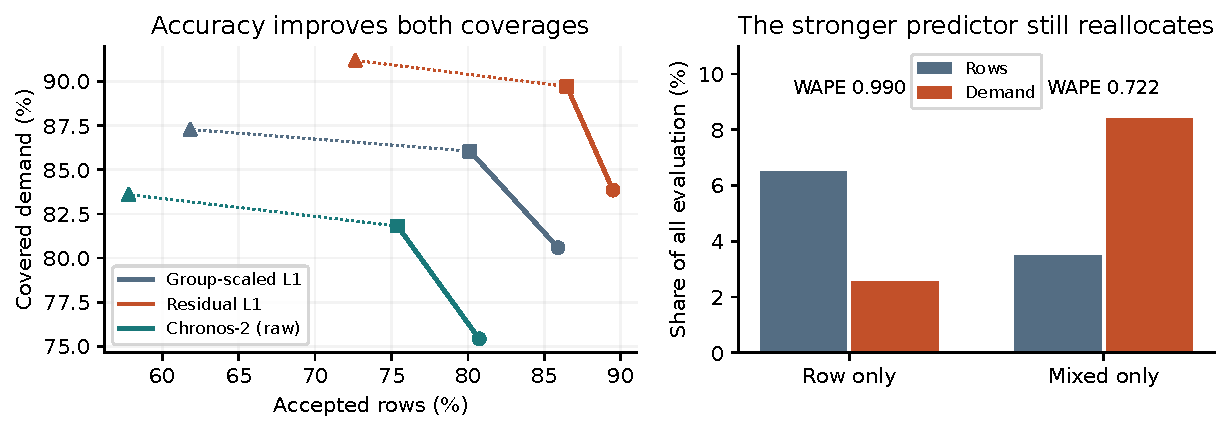
\includegraphics[width=\linewidth]{figures/accuracy_coverage.pdf}
\caption{Matched-date comparison. Left: moving to a stronger predictor raises both coverages, while changing utility within a predictor trades them off. Circles, squares, and triangles denote $\lambda=1,0.25,0$. Lines connect evaluated settings, not Pareto frontiers. Right: the improved predictor's exclusive acceptance sets retain the budget mechanism.}
\label{fig:accuracy}
\end{figure}
The improved mixed policy also exceeds the base row policy in both coverages (86.48/89.72 versus 85.90/80.59 percent). Nevertheless, its row-only set carries just 2.55\% of demand while spending 59.84\% of common slack (Appendix~\ref{app:accuracy}). The smaller case sacrifice (3.02 versus 5.77 points) coexists with the same mechanism. Neither pooled policy establishes the Hobbies or Household cap.
